Как было рассмотрено ранее, информатика изучает знаковые (алфавитные) системы.\\ \textbf{Алгебра} -- наиболее адекватный математический аппарат описания действий в них, поэтому алгебраический аппарат наилучшим образом подходит для описания информационных систем общей природы, отвлеченно от их предметной направленности. Информационные процессы хорошо формализуются с помощью различных алгебраических структур. \\
\\Кроме обычной алгебры существует специальная, основы которой были заложены английским математиком XIX века Дж. Булем. Эта алгебра занимается так называемым исчислением высказываний. Её особенностью является применимость для описания работы так называемых дискретных устройств, к числу которых принадлежит целый класс устройств автоматики и вычислительной техники.
\section{Определение}
\begin{wrapfigure}[13]{l}{2.5cm}
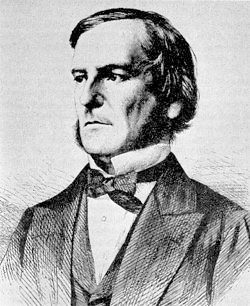
\includegraphics[width=2.5cm]{7_1}
\begin{center}
\caption{}
\footnotesize{Джордж Буль}
\\\footnotesize{$1815 -- 1864$}
\end{center}
\end{wrapfigure}
\textbf{Алгебра двоичной логики} -- раздел математики, в котором изучаются логические операции над высказываниями. Чаще всего предполагается, что высказывания могут быть только истинными или ложными, то есть используется так называемая бинарная или двоичная логика. Один из основателей алгебры логики -- Джордж Буль.
\\
\\\textbf{Логическая (булева) переменная} -- такая переменная, значения которой могут быть лишь <<1>> или <<0>>.
\\\emph{В естественном языке:} <<булева переменная>> $=$ <<высказывание>>.
\\
\textbf{\\Высказывание} -- утверждение, про которое можно однозначно сказать, истинно оно или ложно.
\\\emph{Обозначения:}
\begin{itemize}
  \item <<истина>> \ и <<ложь>>;
  \item <<true>> \ и <<false>>;
  \item <<1>> \ и <<0>>.
\end{itemize}
Например, высказывание <<Москва -- столица России>> -- истина, а <<трава синего цвета>> -- ложь.
\\
\textbf{Логическая (булева) функция $f(x, y, z, …)$} -- некоторая функциональная зависимость, в результате выполнения логических операций над логическими переменными $x, y, z,\dots$ получает значение 0 или 1.
\textbf{Таблица истинности} -- таблица всех значений некоторой \emph{логической функции}.
\begin{center}
  \emph{Основные операции}
\end{center}
\begin{itemize}
\item $\bar{x}$ -- отрицание или инверсия;
\item$x \vee y$ -- дизъюнкция или логическое сложение;
\item$x \wedge y$ -- конъюнкция или логическое умножение;\\
\end{itemize}
Кроме указанных трех базовых операций можно с их помощью ввести еще следующие важные операции алгебры предикатов (можно их назвать небазовыми операциями):\\
\begin{itemize}
\item$(x\to y) \equiv (\bar{x} \vee y)$ -- импликация; \\
\item$(x\leftrightarrow y) \equiv (x \wedge y \vee \bar{x} \wedge \bar{y})$ -- эквиваленция.
\end{itemize}\\
Операции импликации и эквиваленции хотя и часто используются, но не являются базовыми, ибо они определяемы через три введенные выше базовые операции. При выполнении логических операций в компьютере они сводятся к поразрядному сравнению битовых комбинаций. Эти операции достаточно быстро (аппаратно) выполняемы, так как сводятся к выяснению совпадения или несовпадения битов.\\
\\В логических формулах определено старшинство операций, например: скобки, отрицание, конъюнкция, дизъюнкция (остальные, небазовые операции пока не учитываем).\\
\\Всегда истинные формулы называют \textbf{тавтологиями}.\\
\\\emph{Логические функции} эквивалентны, если совпадают их таблицы истинности, то есть совпадают области определения и значения, а также сами значения функции при одних и тех же наборах переменных из числа всех допустимых значений. Если это совпадение происходит на части множества допустимых значений, то формулы называются эквивалентными лишь на этой части (на этом подмножестве).\\
\\Задача \textbf{упрощения логического выражения} состоит в преобразовании его к более простому (по числу переменных, операций или операндов) эквивалентному выражению. Наиболее простой вид получается при сведении функции к постоянной – 1 (истина) или 0 (ложь).


\section{Основные тождества}
\begin{enumerate}
  \item Аксиома двойного отрицания \\
     $$\bar{\bar{x}} = x$$
  \item Аксиома существования 1 и 0 \\
  \begin{minipage}{5cm}
     $$0 = \bar{1}$$
     $$1 = \bar{0}$$
  \end{minipage}
  \begin{minipage}{5cm}
     $$x \vee \bar{x} = 1$$
     $$x \wedge \bar{x} = 0$$
  \end{minipage}
  \item Закон идемпотенции \\
  \begin{minipage}{5cm}
     $$x \vee x = x$$
  \end{minipage}
  \begin{minipage}{5cm}
     $$x \wedge x = x$$
  \end{minipage}
  \item Закон коммутативности \\
  \begin{minipage}{5cm}
     $$x \vee y = y \vee x$$
  \end{minipage}
  \begin{minipage}{5cm}
     $$x \wedge y = y \wedge x$$
  \end{minipage}
  \item Закон поглощения \\
  \begin{minipage}{5cm}
     $$x \vee (x \wedge y) = x$$
  \end{minipage}
  \begin{minipage}{5cm}
     $$x \wedge (x \vee y) = x$$
  \end{minipage}
  \item Закон ассоциативности \\
  \begin{minipage}{5cm}
     $$x \vee (y \vee z) = (x \vee y) \vee z$$
  \end{minipage}
  \begin{minipage}{5cm}
     $$x \wedge (y \wedge z) = (x \wedge y) \wedge z$$
  \end{minipage}
  \item Закон дистрибутивности \\
  \begin{minipage}{5cm}
     $$x \vee (y \wedge z) = (x \vee y) \wedge (x \vee z)$$
  \end{minipage}
  \begin{minipage}{5cm}
     $$x \wedge (y \vee z) = (x \wedge y) \vee (x \wedge z)$$
  \end{minipage}
  \item Законы де Моргана \\
  \begin{minipage}{5cm}
     $$\bar{x \vee y} = \bar{x} \wedge \bar{y}$$
  \end{minipage}
  \begin{minipage}{5cm}
     $$\bar{x \wedge y} = \bar{x} \vee \bar{y}$$
  \end{minipage}
  \item Закон нейтральности \\
  \begin{minipage}{5cm}
     $$x \vee (y \wedge \bar{y}) = x$$
  \end{minipage}
  \begin{minipage}{5cm}
     $$x \wedge (y \vee \bar{y}) = x$$
  \end{minipage}
\end{enumerate}

\section{Таблица истинности}
Существует только 4 различные логические функции одной переменной $F(x)$. Любая другая функция (даже самая сложная вида $F(x) = \bar{x} \vee x \wedge \bar{x}$) будет иметь одну из следующих таблиц истинности:
\begin{table}[!h]
\begin{center} 
\caption{}
\begin{tabular}{|c||c|c|c|c|}
\hline
$x$ & $F_0(x)$ & $F_1(x)$ & $F_2(x)$ & $F_3(x)$ \\
\hline
\hline
0 & 0 & 1 & 0 & 1 \\
\hline
1 & 0 & 0 & 1 & 1 \\
\hline
\end{tabular}
\end{center} 
\end{table}
\\Например $F(x) = \bar{x}$ будет иметь таблицу истинности $F_1(x)$, а $F(x) = 1$ -- $F_3(x).$
\\
\\Обычно логическую функцию $F(x)$ обозначают как $FK,N$, где $K$ -- количество операндов, а $N$ -- число в десятичной системе счисления, которое при переводе в двоичную является таблицей истинности функции. Например, $F(x) = \bar{x}$ обозначается как $F1,2$, так как одна переменная и $2_{10} = 01_{2}$, что является таблицей истинности функции (смотреть снизу вверх).
\\
\\Для $k$ переменных будет существовать $N = 2^{2^{k}}$ функций.
\\Рассмотрим таблицу истинности:
\\
\\
\begin{minipage}{2cm}
\begin{center}
$L$ штук\\
(от 00..0\\ до 11..1 \\ сверху \\ вниз)
\end{center}
\end{minipage}
\begin{minipage}{0.3cm}
\quad \\
\quad \\
$\left\{
\begin{array}{c}
\\
\\
\\
\\
\end{array}
\right.$
\quad \\
\end{minipage}
\begin{minipage}[l]{9cm}

\begin{tabular}{c|c|c|c|c|c|c|c|c|}
\hhline{~--------}
& \multicolumn{4}{c|}{Значения $k$ штук} & \multicolumn{4}{c|}{\multirow{2}{*}{Значение булевых функций $F$}} \\
& \multicolumn{4}{c|}{булевых операндов} & \multicolumn{4}{c|}{}\\
\hhline{~--------}
& $x_1$ & $x_2$ & \dots & $x_k$ & $FK,0$ & $FK,1$ & \dots & $FK,N$ \\
\hhline{~--------}
 & 0 & 0 & \dots & 0 & 0 & 1 & \dots & 1\\
& 0 & 0 & \dots & 1 & 0 & 0 & \dots & 1\\
& \dots & \dots & \dots & \dots & \dots & \dots & \dots & \dots\\
\multirow{4}{*}{} & 1 & 1 & \dots & 1 & 0 & 0 & \dots & 1\\

\hhline{~--------}
\multicolumn{5}{c}{} & \multicolumn{4}{c}{$\underbrace{\qquad \qquad \qquad \qquad \qquad \qquad \qquad}_{\mbox{от N штук (от 00..0 }}$} \\
\multicolumn{5}{c}{} & \multicolumn{4}{c}{до 11..1 слева направо)}
\end{tabular}
\end{minipage}
\\
\\
\\
Так как всего $k$ переменных, то для них будет $L = 2^k$ строк в таблице истинности, а количество булевых функций будет равно $N = 2^L$. Отсюда:
\\
\begin{center}
\begin{tabular}{c c}
$L = 2^k$ & \multirow{2}{*}{$\Rightarrow N = 2^{2^{k}}$} \\
$N = 2^L$ & \\
\end{tabular}
\end{center}
Так, для 1 переменной будет 4 булевых функции, для 2 переменных -- 16 и так далее.
\newpage
\begin{table}[!h]
\caption{Таблица значений и названий булевых функций от двух переменных}
\begin{tabular}{|c|c|c|c|c|c|c|}
\hline
$x$ & 1 & 1 & 0 & 0 & \multirow{2}{*}{Обозначение} & \multirow{2}{*}{Название} \\
\hhline{------~~}
$y$ & 1 & 0 & 1 & 0 & & \\
\hline
\multirow{2}{*}{F} & \multirow{2}{*}{0} & \multirow{2}{*}{0} & \multirow{2}{*}{0} & \multirow{2}{*}{0} & F2,0 = $FALSE$  & Противоречие,  \\
& & & & & & логичечский нуль \\
\hline
\multirow{3}{*}{F} & \multirow{3}{*}{0} & \multirow{3}{*}{0} & \multirow{3}{*}{0} & \multirow{3}{*}{1} & F2,1 = $x\downarrow y = x NOR y = $  & Cтрелка Пирса, НЕ--ИЛИ, \\
& & & & & $= NOR(x,y) = x $НЕ--ИЛИ & антидизъюнкция \\
& & & & & $y = $НЕ--ИЛИ$(x,y)$ & \\
\hline
\multirow{2}{*}{F} & \multirow{2}{*}{0} & \multirow{2}{*}{0} & \multirow{2}{*}{1} & \multirow{2}{*}{0} & F2,2 = $x\leftarrow /y$  & Отрицание \\
& & & & & & обратной импликации \\
\hline
\multirow{1}{*}{F} & \multirow{1}{*}{0} & \multirow{1}{*}{0} & \multirow{1}{*}{1} & \multirow{1}{*}{1} & F2,3 = $\neg x $  &  Отрицание\\
\hline
\multirow{3}{*}{F} & \multirow{3}{*}{0} & \multirow{3}{*}{1} & \multirow{3}{*}{0} & \multirow{3}{*}{0} & F2,4 = $x\rightarrow /y $  & Материальная \\
& & & & & & обратная импликация \\
\hline
\multirow{1}{*}{F} & \multirow{1}{*}{0} & \multirow{1}{*}{1} & \multirow{1}{*}{0} & \multirow{1}{*}{1} & F2,5 = $ \neg y$  & Отрицание \\
\hline
\multirow{4}{*}{F} & \multirow{4}{*}{0} & \multirow{4}{*}{1} & \multirow{4}{*}{1} & \multirow{4}{*}{0} & F2,6 =  $x \oplus y$ = & Сложение по модулю 2, \\
& & & & & = $x XOR y = XOR(x,y)$ = & исключающее "или" \\
& & & & & = $x >< y = x <> y$ = & сумма Жегалкина, \\
& & & & & = $x NE y = NE(x,y)$ & не равно \\
\hline
& & & & & F2,7  = x | y = & Штрих Шеффера, \\
F & 0 & 1 & 1 & 1 & = $NAND(x,y)$ = $x NAND$ & НЕ--И, 2И--НЕ, \\
& & & & & $y$ = $x$ НЕ--И $y$ = НЕ--И$(x,y)$ & антиконъюнкция\\
\hline
& & & & & F2,8 = $x \wedge y = x \cdot y =$ &  \\
\multirow{2}{*}{F} & \multirow{2}{*}{1} & \multirow{2}{*}{0} & \multirow{2}{*}{0} & \multirow{2}{*}{0} &  = $xy = x \& y = x AND y$ = & Конъюнкция,\\
& & & & & = $AND(x,y) = x $И$ y =$ & 2И, минимум \\
& & & & & = И$(x,y) = min(x,y)$	& \\
\hline
& & & & & F2,9 = $(x \equiv y) = x ~ y $= & Эквивалентность \\
F & 1 & 0 & 0 & 1 & = $x \leftrightarrow y = x EQV y = $ & равенство\\
& & & & & = $EQV(x,y)$ & \\
\hline
\multirow{1}{*}{F} & \multirow{1}{*}{1} & \multirow{1}{*}{0} & \multirow{1}{*}{1} & \multirow{1}{*}{0} & F2,10 = $y $  & Проекция, повторение\\
\hline
\multirow{2}{*}{F} & \multirow{2}{*}{1} & \multirow{2}{*}{0} & \multirow{2}{*}{1} & \multirow{2}{*}{1} & F2,11 = $x \to y = x  \supset y$ = & Импликация \\
& & & & &  = $x \le y = x LE y = LE(x,y)$ & следование  \\
\hline
\multirow{1}{*}{F} & \multirow{1}{*}{1} & \multirow{1}{*}{1} & \multirow{1}{*}{0} & \multirow{1}{*}{0} & F2,12 = $x $  & Проекция, повторение\\
\hline
\multirow{1}{*}{F} & \multirow{1}{*}{1} & \multirow{1}{*}{1} & \multirow{1}{*}{0} & \multirow{1}{*}{1} & F2,13 = $x \leftarrow y $  & Обратная импликация\\
\hline
& & & & & F2,14 = $x \vee y = x + y =$ &  \\
\multirow{2}{*}{F} & \multirow{2}{*}{1} & \multirow{2}{*}{1} & \multirow{2}{*}{1} & \multirow{2}{*}{0} & =$ x OR y = OR(x,y) = $ & Дизъюнкция,\\
& & & & & = $x$ ИЛИ $y$ = ИЛИ$(x,y)$ = & 2ИЛИ, максимум \\
& & & & & $ = max(x,y)$	& \\
\hline
\multirow{1}{*}{F} & \multirow{1}{*}{1} & \multirow{1}{*}{1} & \multirow{1}{*}{1} & \multirow{1}{*}{1} & F2,15 = $TRUE $  & Тавтология\\
\hline
\end{tabular}

\end{table}
\newpage
\section{Обозначение на электрической схеме булевых функций}
Для аппаратной реализации булевых функций и их корректного обозначения на электрической схеме принято использовать логические элементы.
\\
\\\textbf{Логический элемент} – это простейшее устройство ЭВМ, выполняющее одну определенную логическую операцию над входными сигналами согласно правилам алгебры логики. То есть, одну из функций, рассмотренных ранее.\\
\textbf{Рассмотрим современные стандарты для условных графических обозначений (УГО) логических элементов:}

\begin{itemize}
  \item ANSI (англ.\emph{American national standards institute} -- американский национальный институт стандартов);
  \item MIL/IEC (англ.\emph{MILitary} – военный, {International Electrotechnical Commission} -- международная электротехническая комиссия);
  \item DIN (нем. \emph{Deutsches Institut f{\"u}r Normung e. V.} — немецкий институт по стандартизации);
  \item ГОСТ 2.743--91, Единая система конструкторской документации. Обозначения условные графические в схемах. Элементы цифровой техники. 
\end{itemize}
\begin{table}[!h]
\centering
\caption{Обозначение некоторых булевых функций на электросхеме}
\begin{tabular}{|c|c|c|c|}
\hline
Название & IEC & ANSI \\
\hline
\multirow{3}{*}{НЕ, $\bar{A}$ (Инвертор)} & \multirow{3}{*}{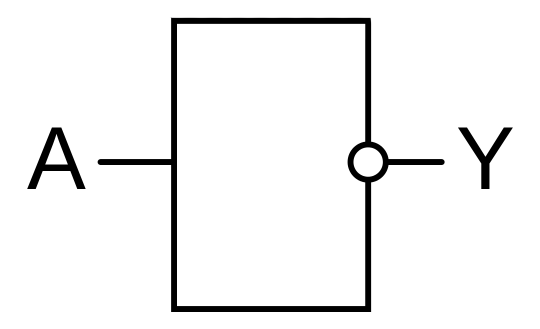
\includegraphics[width=2cm]{7_2(1)}} & \multirow{3}{*}{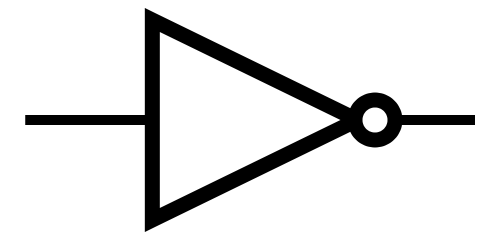
\includegraphics[width=2cm]{7_2(2)}} \\
& & \\
& & \\
\hline
\multirow{3}{*}{И, $A \wedge B$} & \multirow{3}{*}{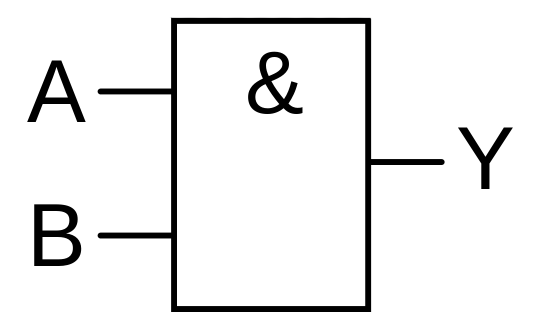
\includegraphics[width=2cm]{7_3(1)}} & \multirow{3}{*}{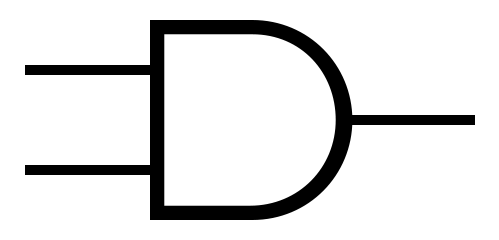
\includegraphics[width=2cm]{7_3(2)}} \\
& & \\
& & \\
\hline
\multirow{3}{*}{ИЛИ, $A \vee B$} & \multirow{3}{*}{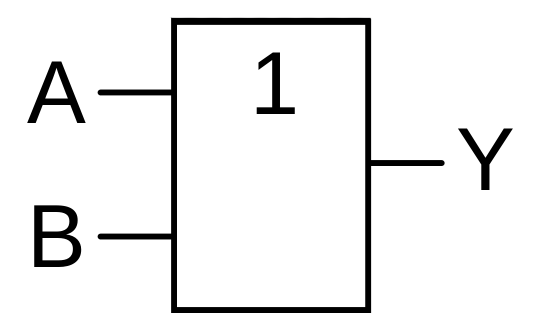
\includegraphics[width=2cm]{7_5(1)}} & \multirow{3}{*}{
\includegraphics[width=2cm]{7_5(2)}} \\
& & \\
& & \\
\hline
\multirow{3}{*}{Сумма по модулю 2, $A \oplus B$} & \multirow{3}{*}{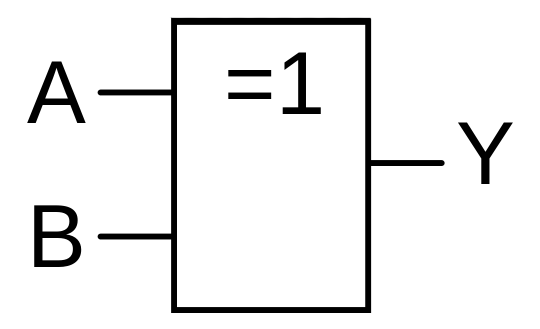
\includegraphics[width=2cm]{7_4(1)}} & \multirow{3}{*}{
\includegraphics[width=2cm]{7_4(2)}} \\
& & \\
& & \\
\hline
\end{tabular}

\end{table}
%\begin{minipage}{\textwidth}
Это основные обозначения. Они могут совмещаться. Например, так будет выглядеть И--НЕ:
\\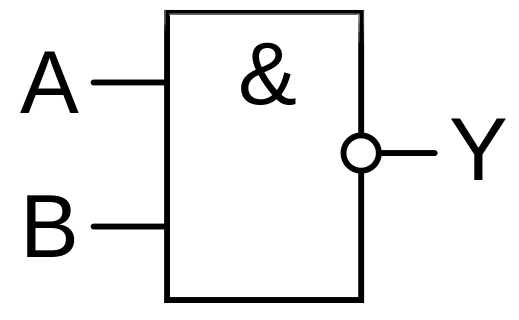
\includegraphics[width=2cm]{7_6}
%\end{minipage}
\\
\\\textbf{Цена функции по Квайну} – суммарное число входов логических элементов в составе схемы.
\\\textbf{Минимизация функции} – сокращение цены функции, с помощью преобразования её к более простому эквивалентному выражению.
Наиболее простой вид получается при сведении функции к постоянной -- 1 (истина) или 0 (ложь).
\section{Логический базис}
\textbf{Логический базис} -- набор булевых функций, позволяющий реализовать любую другую булеву функцию.
\\Три наиболее востребованных логических базиса: И, ИЛИ, НЕ; ИЛИ--НЕ; И--НЕ.
\begin{figure}[!h]
\centering
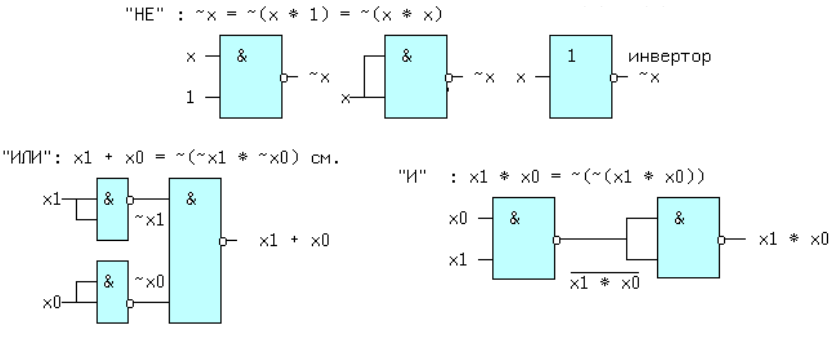
\includegraphics[width=\textwidth]{7_7}
\caption{Пример реализации функций И, ИЛИ, НЕ в базисе И--НЕ}
\end{figure}
\section{Формы записи математических выражений}
Форма записи по--другому называется нотацией.
\\"Арность операции" означает количество операндов, участвующих в операции.
\\Например: $\sqrt{A}$ (унарная), $A\times B$ (бинарная).
\\
\begin{center}
 \textbf{Виды нотаций}
\end{center}
\begin{itemize}
  \item[1489 г.] -- инфиксная запись $A + B$;
  \item[1920 г.] -- префиксная (польская) запись $+AB$;
  \item[1957 г.] -- постфиксная (обратная польская) запись $AB+$.
\end{itemize}
\textbf{Стек} -- абстрактный тип данных, представляющий собой список элементов, организованных по принципу LIFO (англ. \emph{last in -- first out}, "последним пришел -- первым вышел"). Чаще всего принцип работы стека сравнивают со стопкой тарелок: чтобы взять вторую сверху, нужно снять верхнюю.
\subsection{Префиксная нотация}
\textbf{\emph{Пример:}}
\\Инфиксная нотация: $(A + B + C) -- E^{D\times F\times G}.$
\\Префиксная нотация: $--++ABC^{\wedge}E\times\times DFG.$
\\
\\Рассмотрим, как же происходит запись в префиксной нотации:
\begin{enumerate}
 \item Исходное выражение: $(A + B + C) -- E^{D\times F\times G}$. Расставляем порядок выполнения операций, согласно математическим правилам.
\item Последним выполняется вычитание, а именно из $(A + B + C)$ вычитается $E^{D\times F\times G}$. \textbf{Ставим знак в начало.} Получается $--(A + B + C)(E^{D\times F\times G})$.
\item Рассмотрим $(A + B + C)$, расставим порядок действий. Сначала происходит сложение $A$ и $B$, а потом $A+B$ и $C$. Начнем с последнего действия, получается: $+(A+B)C$. В $(A+B)$ происходит сложение $A$ и $B$, получаем $(+AB)$. Совместим все вместе: $(+(+AB)C)$.
\item Рассмотрим $(E^{D\times F\times G})$, происходит возведение в степень. А именно $E$ возводится в степень $D\times F\times G$. Получается $^{\wedge}E(D\times F\times G)$.
\item Рассмотрим $D\times F\times G$, расставляем порядок действий. Сначала происходит умножение $D$ и $F$, а потом $D\times F$ и $G$. Начнем с последнего действия, получается: $\times(D \times F)G$. В $(D \times F)$ происходит умножение $D$ и $F$, получаем $(\times DF)$. Совместим все вместе: $(\times(\times DF)G)$.
\item Совмещаем все вместе. Получается: $--(+(+AB)C)(^{\wedge}E(\times(\times DF)G)$. Убираем скобки. Получили $--++ABC^{\wedge}E\times\times DFG$.
\end{enumerate}
Существует популярная Lisp--разновидность префиксной нотации (Lisp -- семейство языков программирования). И в ней запись будет выглядеть так: $(--(+ABC)(^{\wedge}E(\times DFG))).$
\begin{center}
  \textbf{Особенности префиксной нотации}
\end{center}
\begin{itemize}
  \item Не требуется скобок, если арность фиксирована;
  \item Запись выражения получается короче, чем инфиксная;
  \item Не требуется знать приоритет операций;
  \item Легко декодировать выражение с помощью стека;
  \item Малоприменима на практике (кроме Lisp).
\end{itemize}
\subsection{Постфиксная нотация}
\textbf{\emph{Пример 1:}}
\\Инфиксная нотация: $(A + B + C) -- E^{D\times F\times G}$
\\Постфиксная нотация: $CAB++EGDF\times\times ^{\wedge}--$
\\
\par\textbf{\emph{Пример 2:}}
\\Инфиксная нотация:$ ( A + B ) \items ( C + D )$
\\Постфиксная нотация: $A B + C D + \times$
\\
\\Рассмотрим, как же происходит запись в постфиксной нотации:
\begin{enumerate}
\item Исходное выражение: $(A + B + C) -- E^{D\times F\times G}$. Расставляем порядок выполнения операций, согласно математическим правилам.
\item Последним выполняется вычитание, а именно из $(A + B + C)$ вычитается $E^{D\times F\times G}$. Ставим знак в конец. Получается $(A + B + C)(E^{D\times F\times G})--$.
\item Рассмотрим $(A + B + C)$, расставим порядок действий. Сначала происходит сложение $A$ и $B$, а потом $A+B$ и $C$. Начнем с последнего действия, получается: $С(A+B)+$. В $(A+B)$ происходит сложение $A$ и $B$, получаем $(AB+)$. Совместим все вместе: $(C(AB+)+)$.
\item Рассмотрим $(E^{D\times F\times G})$, происходит возведение в степень. А именно $E$ возводится в степень $D\times F\times G$. Получается $E(D\times F\times G)^{\wedge}$.
\item Рассмотрим $D\times F\times G$, расставляем порядок действий. Сначала происходит умножение $D$ и $F$, а потом $D\times F$ и $G$. Начнем с последнего действия, получается: $G(D \times F)\times$. В $(D \times F)$ происходит умножение $D$ и $F$, получаем $(DF\times)$. Совместим все вместе: $(G(DF\times )\times)$.
\item Совмещаем все вместе. Получается: $(C(AB+)+)(E(G(DF\times)\times)^{\wedge})--$. Убираем скобки. Получили $CAB++EGDF\times\times ^{\wedge}--$.
\end{enumerate}
\begin{center}
  \textbf{Особенности постфиксной нотации}
\end{center}
\begin{itemize}
  \item Не требуется скобок, если арность фиксирована;
  \item Запись выражения получается короче, чем инфиксная;
  \item Не требуется знать приоритет операций;
  \item Легко декодировать выражение с помощью стека;
  \item Успешно применяется в компиляторах, в небольшом количестве языков программирования и некоторых ЭВМ (калькуляторы "Электроника" и HP).
\end{itemize}
\begin{center}
  \textbf{Алгоритм вычисления для постфиксной нотации}
\end{center}
\begin{enumerate}
  \item Обработка входного символа:
  \begin{itemize}
    \item Если на вход подан операнд, он помещается на вершину стека;
    \item Если на вход подан знак операции, то соответствующая операция выполняется над требуемым количеством значений, извлеченных из стека, взятых в порядке добавления. Результат выполненной операции кладется на вершину стека.
  \end{itemize}
  \item Если входной набор символов обработан не полностью, перейти к шагу 1.
  \item После полной обработки входного набора символов результат вычисления выражения лежит на вершине стека.
\end{enumerate}

%todo из онлайн курса текст дописать
\begin{figure}[h]
\centering
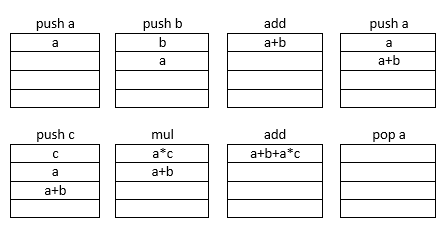
\includegraphics[width=\textwidth]{7_8}
\caption{Вычисления выражения $ab+ac\times +$ (в инфиксной нотации $a\hm+b\hm+a\times c$)}
\end{figure}
Рассмотрим вычисление постфиксной нотации в стеке. Стек не имеет адресных операций. В нем есть две операции с переменными: $push$ (положить) и $pop$ (забрать). Если необходимо положить значение в стек, то он кладется с помощью команды $push$ на вершину стека. При этом, все другие значения сдвигаются вниз. Арифметические операции ($add$ -- сложить, $mul$ -- умножить) выполняются с переменными (или переменной -- зависит от арности операции), которые лежат на вершине стека.